\documentclass[xcolor=dvipsnames]{beamer}

% Packages
\usepackage{bm}
\usepackage{wasysym}


%% Theme related.
\usetheme{default}
\setbeamerfont{author}{size = \large}
\setbeamerfont{institute}{size=\large}
\setbeamerfont{footline}{series = \bfseries}
\setbeamertemplate{navigation symbols}{}
\setbeamertemplate{frametitle}[default][center]
\setbeamertemplate{itemize items}[circle]
\definecolor{Red}{rgb}{.9,.05,.05}
\setbeamercolor{alerted text}{fg=Red}
\usefonttheme[onlymath]{serif}


%% Math
\newcommand{\Reals}{\mathbb{R}}
\newcommand{\wh}[1]{\widehat{#1}}
\newcommand{\wt}[1]{\widetilde{#1}}
\DeclareMathOperator*{\argmin}{argmin}

%% Font
\newcommand{\red}[1]{\textcolor{red}{#1}}
\newcommand{\blue}[1]{\textcolor{blue}{#1}}

\title{Minimax Optimality of Laplacian Smoothing}
\subtitle{\small (Full title: Minimax Optimal Regression over Sobolev Spaces via Laplacian Regularization on Neighborhood Graphs)}

\author{Alden Green, Sivaraman Balakrishnan, Ryan Tibshirani}
\institute{Department of Statistics and Data Science \\

\includegraphics[width=.5 \textwidth]{figures/cmu.png}}
\date{}

\begin{document}
	
\begin{frame}
\titlepage
\end{frame}

\addtobeamertemplate{navigation symbols}{}{
	\usebeamerfont{footline}
	\usebeamercolor[fg]{footline}
	\hspace{1em}
	\insertframenumber
}
\addtocounter{framenumber}{-1}

\begin{frame}{Basic problem setup}
\alert{Nonparametric regression, random design}: We observe $(X_1,Y_1),\ldots,(X_n,Y_n)$, where $X_1,\ldots,X_n \in \Reals^d$ are sampled independently from density $p$, and
\begin{equation*}
Y_i = f_0(X_i) + \varepsilon_i, \quad \varepsilon_i \sim N(0,1).
\end{equation*}
Goal is to estimate the unknown regression function $f_0$, which is assumed to be \alert{Sobolev} smooth, i.e.
\begin{equation*}
\|f_0\|_{H^1}^2 := \int \|\nabla f_0(x)\|^2 \,dx \quad \text{is small.}
\end{equation*}
\end{frame}

\begin{frame}{Laplacian smoothing}
Laplacian smoothing solves a discrete, penalized least squares problem on a graph.
\pause
\begin{enumerate}
	\item  Form a \alert{neighborhood graph} $G$ over $X_1,\ldots,X_n$, with weighted edges $W_{ij} = K(\|X_i - X_j\|/r)$. The \alert{graph Laplacian} $L = D - W$ induces a semi-norm,
	\begin{equation*}
	f^{\top} L f = \sum_{i,j = 1}^{n} \bigl(f(X_i) - f(X_j)\bigr)^2 W_{ij}.
	\end{equation*}
	\pause
	\item The \alert{Laplacian smoothing} estimator is
	\begin{equation*}
	\wh{f} = \argmin_{f \in \Reals^n} \|Y - f\|_n^2 + \frac{\rho}{2} f^{\top} L f.
	\end{equation*}
	%with corresponding test statistic $\wh{T} = \|\wh{f}\|_n^2$.
\end{enumerate}
\begin{figure}
	\centering
	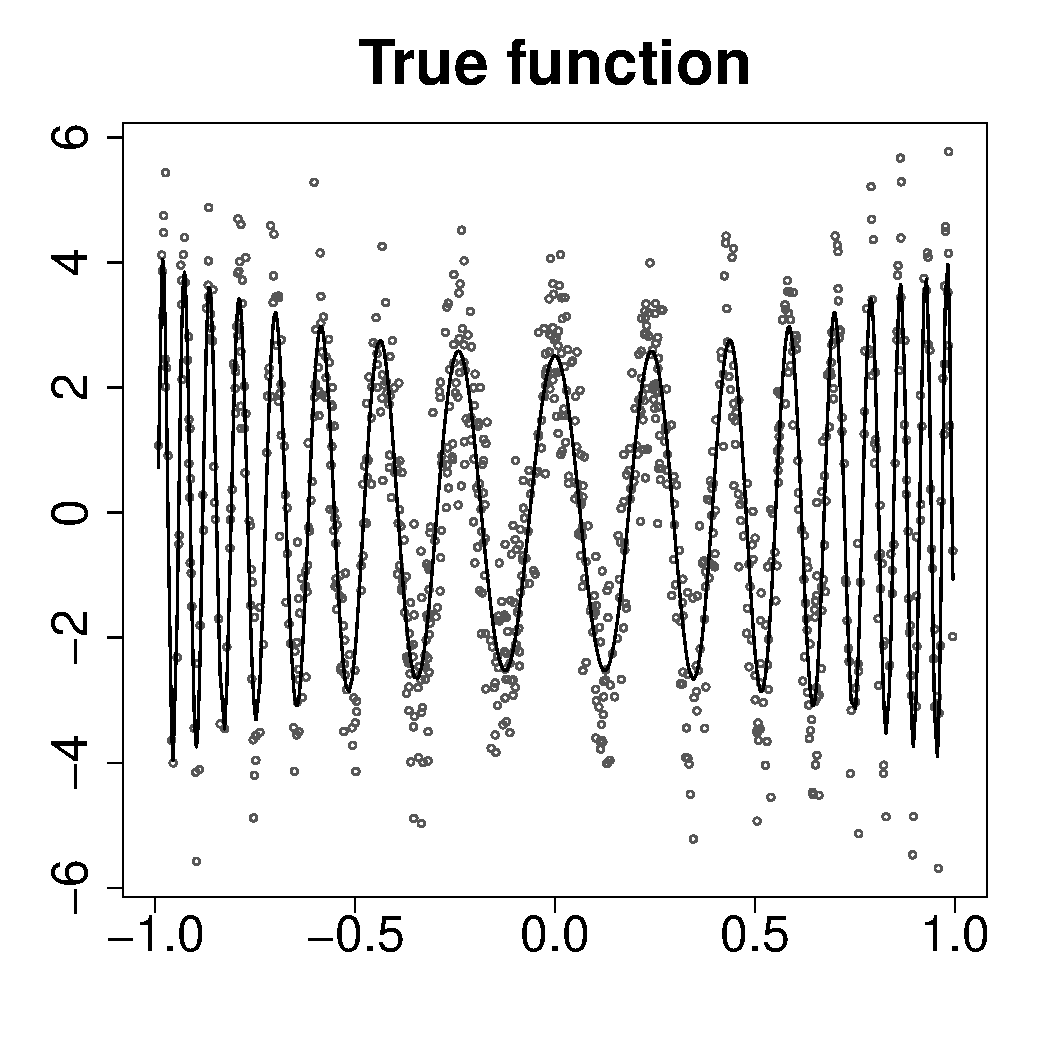
\includegraphics[width=.25\textwidth]{figures/wiggly_cosine/regression_function_1.pdf}
	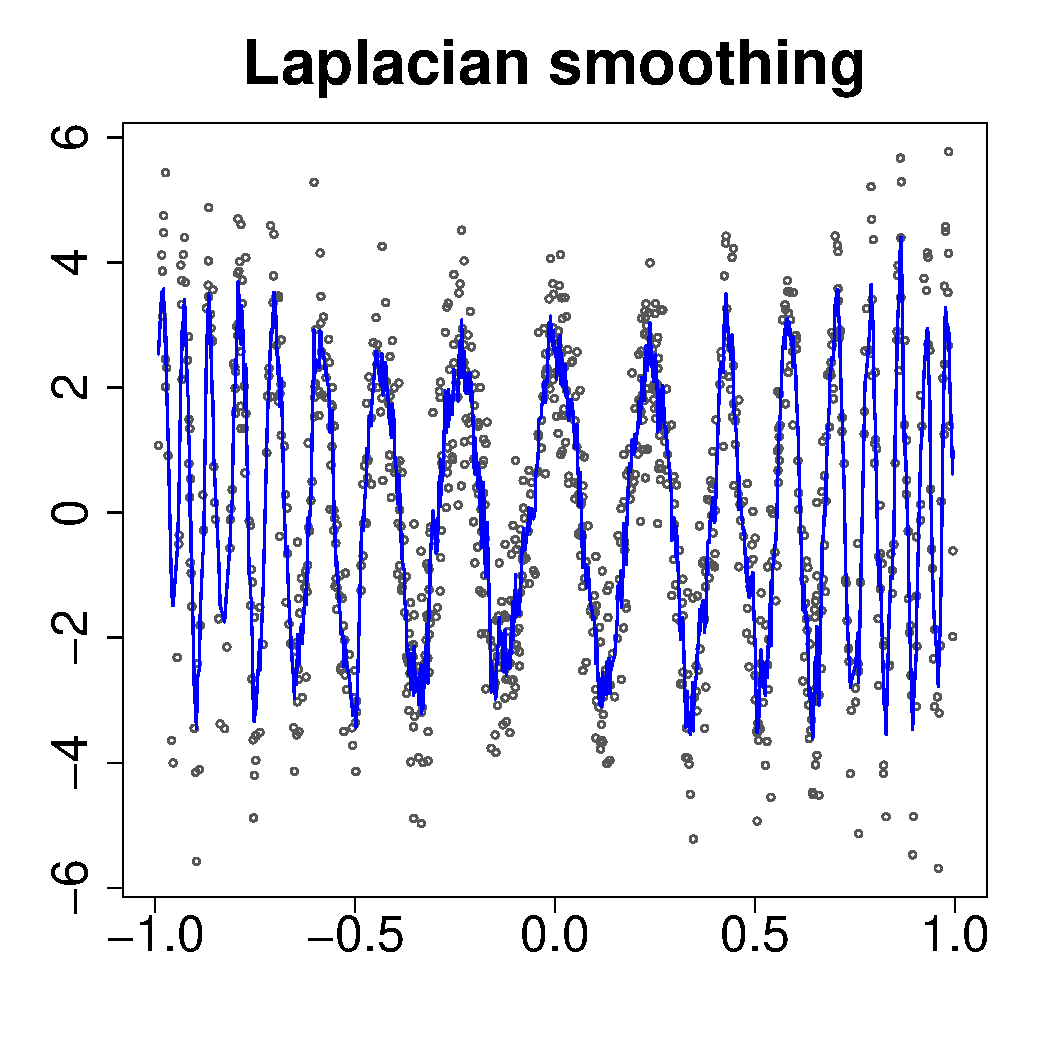
\includegraphics[width=.25\textwidth]{figures/wiggly_cosine/laplacian_smoothing_estimate_1.pdf} 
\end{figure}
\end{frame}

\begin{frame}{Why Laplacian smoothing?}
Intuition: when $p$ uniform, $n$ large, $r$ small and $f$ smooth, {(Bousquet et al. 2004)} show
\begin{equation*}
f^{\top} L f = \frac{1}{2}\sum_{i,j = 1}^{n} \bigl(f(X_i) - f(X_j)\bigr)^2 W_{i,j} \approx n^2 r^{d + 2} \int \|\nabla f(x)\|_2^2 \,dx.
\end{equation*}
\pause
So $\wh{f}$ seems like a noisy and discrete approximation to $\wt{f}$,
\begin{equation*}
\widetilde{f} := \argmin_{f \in H^1} \|Y - f\|_n^2 + \rho \int \|\nabla f(x)\|_2^2  \,dx.
\end{equation*}
Very classical estimator! Aka \alert{smoothing spline} ($d = 1$), or \alert{thin-plate spline} ($d \geq 2$).
\end{frame}

\begin{frame}{Main Question}
In $1d$, smoothing splines achieve the minimax optimal rate \blue{$n^{-2/3}$} (estimation) over Sobolev functions.
\pause
\begin{block}{{\bf Question}}
	Does Laplacian smoothing enjoy the same optimality properties as smoothing/thin plate splines?
\end{block}
\pause
\begin{block}{{\bf Answer}}
	They actually do better! When properly tuned:
	\begin{itemize}
		\item Laplacian smoothing has error of \blue{$n^{-2/3}$}  when $d = 1$, matching smoothing splines.
		\item Laplacian smoothing also achieves optimal error \blue{$n^{-2/(2 + d)}$} when $d = 2,3,4$ (up to $\log n$ factor when $d = 4$).
		\item On the other hand $\wt{f}$ is \alert{not even well-defined} when $d > 1$. Well known in spline/semi-supervised learning communities.
	\end{itemize}
\end{block}
\end{frame}

\begin{frame}{Summary of Main Results}

{\large Estimation rates, assuming $f_0 \in H^1(M)$}
\begin{table}
	\begin{center}
		\begin{tabular}{p{.25\textwidth} | p{.25\textwidth} p{.25\textwidth} }
			Dimension & Laplacian smoothing & Smoothing/Thin-plate splines \\
			\hline
			$d = 1$ & \blue{\bm{${n^{-2/3}}$}} & \blue{${n^{-2/3}}$} \\
			$d = 2,3$ & \blue{\bm{${n^{-2/(2 + d)}}$}} & \red{NA} \\
			$d = 4$ & $\bm{\blue{{n^{-1/3}}} (\log n)^{1/3}}$ & \red{NA} \\
			$d \geq 5$  & $\bm{(\log n/n)^{4/(3d)}}$ & \red{NA} \\
		\end{tabular}
	\end{center}
\end{table}
\end{frame}

\begin{frame}{Extensions}
Several different directions.
\begin{itemize}
	\item \alert{Goodness-of-fit testing}: Use statistic $\wh{T} = \|\wh{f}\|_n^2$ to test whether $f_0 = 0$. Do we achieve optimal rates \blue{$n^{-4/(4 + d)}$}? \blue{(Yes! See paper.)}
	\item \alert{Manifold adaptivity}: When $p$ has support on a manifold of dimension $m < d$, optimal rates are \blue{$n^{-2/(2 + m)}$} (estimation) and \blue{$n^{-4/(4 + m)}$} (testing). Does Laplacian smoothing automatically adapt? \blue{(Yes! See paper.)} 
	\item \alert{Out-of-sample estimation}: Can we extend estimator $\wh{f}$ to have optimal out-of-sample mean squared error? \blue{(Yes, if $f_0$ is Lipschitz! See paper.)}
\end{itemize}
\end{frame}

\begin{frame}[t]{Summary}
	Specific takeaway: Laplacian smoothing is an optimal method for nonparametric regression. \newline
	
	General takeaway: Discretization can allow us to solve problems even when continuum analogues are not well-posed.
	\newline 
	\newline
	\newline
	\pause
	\begin{center}
	{\huge Thank You!}
	\end{center}
	
	
\end{frame}

\begin{frame}{Analysis}
We use a conditional-on-design \alert{bias-variance} decomposition, based on the eigenvalues $\lambda_k$ of $L$. \newline

For estimation,
\begin{equation*}
\|\wh{f} - f_0\|_n^2 \lesssim \rho \frac{f_0^{\top} L f_0}{n} + \frac{1}{n} \sum_{k = 1}^{n} \frac{1}{(\rho \lambda_k + 1)^2}.
\end{equation*}

For testing, level-$\alpha$ test $\varphi = 1\{\wh{T} \geq t_{\alpha}\}$ has negligible Type II error when
\begin{equation*}
\|f_0\|_n^2 \gtrsim \rho \frac{f_0^{\top} L f_0}{n} + \frac{1/\sqrt{\alpha}}{n} \sum_{k = 1}^{n} \sqrt{\frac{1}{(\rho \lambda_k + 1)^4}}.
\end{equation*}

Then we make use of some recent results (Burago et al. 2014, Garcia Trillos et al. 2019) on convergence of eigenvalues $\lambda_k$, and derive some of our own.
\end{frame}

\begin{frame}{What about $d > 4$?}
\alert{Estimation}: the class $H^1(G;M) = \{f: f^{\top}Lf \leq M\}$ is too large to show $\wh{f}$ is optimal. Similar phenomena in ERM over H\"{o}lder classes when $d > 2$ {(Birge and Massart 1993)}, and fixed (grid) graphs {(Sadhanala et al. 2016)}. Empirically, we see that for $f_0$ simple $\cos$ function,
\begin{figure}[tb]
	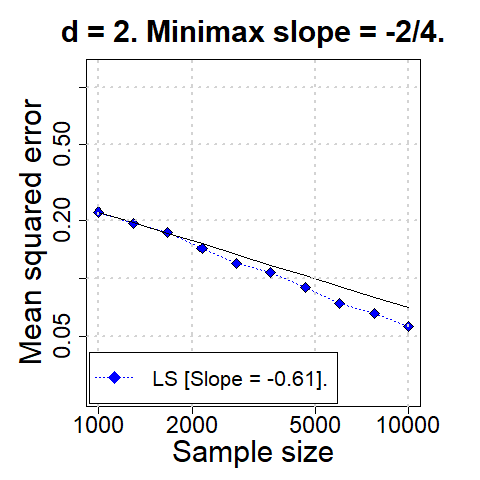
\includegraphics[width=.24\textwidth]{figures/cosine/mse_by_sample_size_2d.png}
	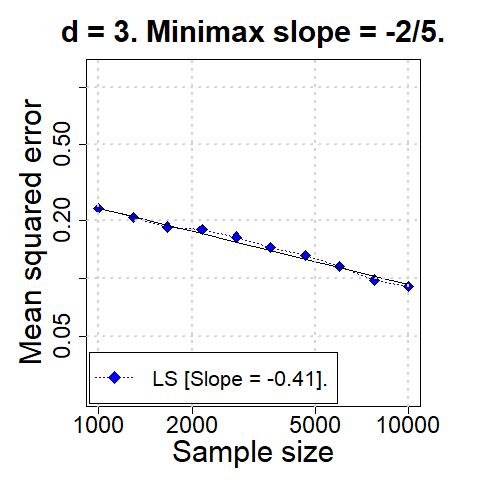
\includegraphics[width=.24\textwidth]{figures/cosine/mse_by_sample_size_3d.png} 
	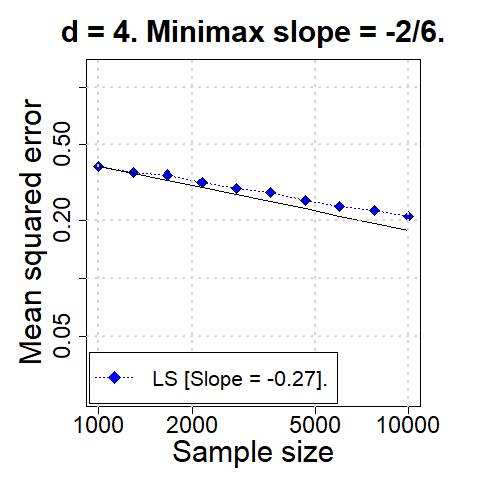
\includegraphics[width=.24\textwidth]{figures/cosine/mse_by_sample_size_4d.png}
	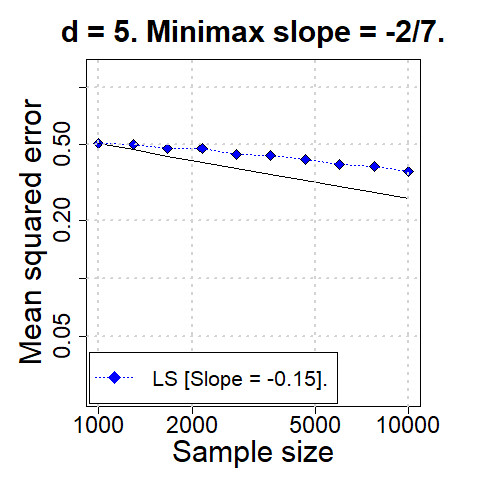
\includegraphics[width=.24\textwidth]{figures/cosine/mse_by_sample_size_5d.png}
\end{figure}

\alert{Testing}: Sobolev class $H^1$ does not embed into $L^4$ (Sobolev Embedding Theorem). Usual test statistics may not have a variance.
\end{frame}

\begin{frame}{Motvation (ctd.)}
Why Laplacian smoothing?
\begin{itemize}
	\item \emph{Computational ease.} Sparse graph, fast solvers.
	\item \emph{Generality.} Makes sense whenever one can form a graph $G$. 
	\item \emph{Weak supervision.} Naturally extends to semi- and unsupervised problems.
\end{itemize}
\pause
\end{frame}



\end{document}
